% Sequential IMPLEMENTATION
\chapter{Sequential implementation}
\label{sequential}
In order to better understand the algorithm, we have started with a basic sequential implementation of it in C++. While this step could be done in any language, we have chosen to work with C++, as it would allow us to re-use pieces of the code for the parallel CUDA implementations, described further in this paper. Running this version with a large number of options will likely result in a significant amount of computation time, however, the purpose of this implementation is rather a proof of concept that the algorithm produces correct approximations, as well as to provide a set of results, which can be used to test against with the other implementations. The sequential implementation code can be found under (TODO: INSERT CODE LOCATION HERE).

The algorithm described in the book is used to price one option at a time and the natural way to start a sequential implementation would be to create a single function that prices one option. Looping through all options in the data set and calling this function for each of them will then produce the end results. The pseudo-code below describes the approach we took for implementing a sequential version of the algorithm, based on the book and articles by Hull and White. Note that real is a data type that can either take the form of a double or a float, based on the necessary precision.

The implementation iterates through all the options, constructs a trinomial tree for each of them and propagates back through it, obtaining the price approximations for each option and returning them in the end. The algorithm follows the intuition provided in the previous section - \ref{section:algorithm_and_intuition}.
    
As it can be seen from the pseudo-code, both the forward propagation and the backward propagation can be done differently, by applying combinations of scatter and gather. Despite that, a gather should always be preferable when dealing with parallelization, due to the reduced number of writes. It can prevent data races between threads and help improve the performance. The intuition behind this can be explained visually, as shown on fig. \ref{fig:scattervsgather}. A scatter can be characterized with reading values out of nodes reading their values and separately writing them to the same location, aggregating to its value. In the scatter example shown (left), a write operation (denoted with blue arrows) is performed from the three nodes (denoted with blue circles) to the same node, thus a total of 3 writes and 3 reads. A gather on the other hand happens when the values are read and aggregated together in one place. That is, on the right figure, the iterator is placed on mid right node, where three read operations are done (denoted with blue arrows), aggregated and followed by one write to the current node (denoted as with blue circle).

(TODO: MABYE WE SHOULD ALSO REPLACE THE SCATTER WITH GATHER ON THE SEQUENTIAL IMPL. AND SEE IF THAT GIVES ANY SPEEDUP BECAUSE OF THE WRITES? EVEN THOUGH WE DON'T CARE MUCH ABOUT THE SEQUENTIAL, OR MOVE THIS SECTION TO MULTIPLE OPTIONS PER THREAD BLOCK)

\begin{figure}[H]
	\centering
	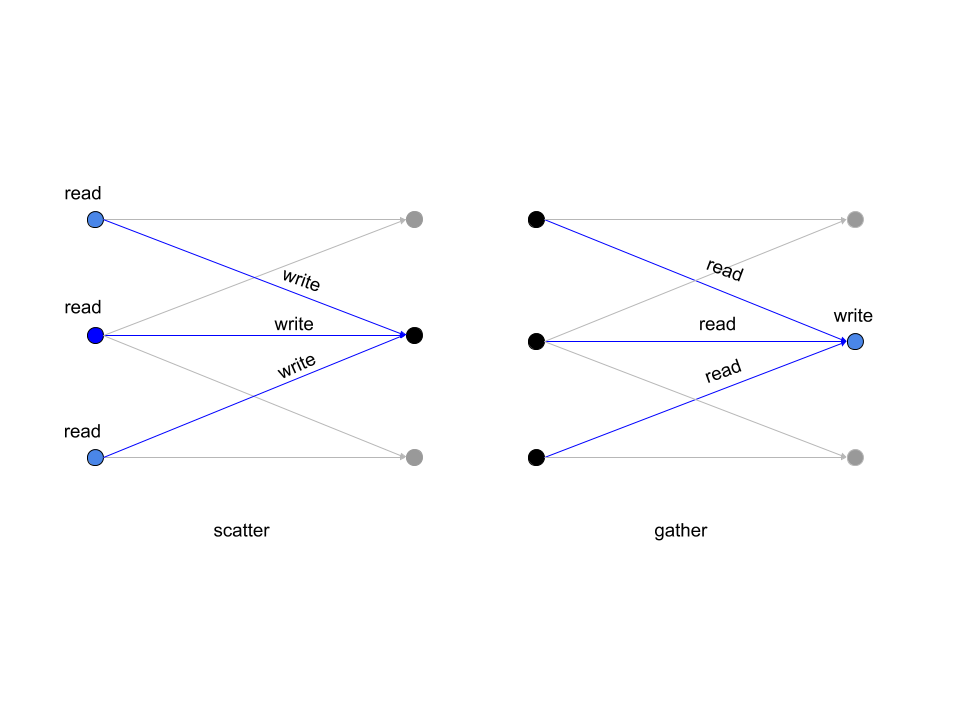
\includegraphics[width=0.8\textwidth]{img/scattervsgather.png}
	\caption{scatter vs. gather operations Source: Compiled by the authors}
	\label{fig:scattervsgather}
\end{figure}

(TODO: WRITE ABOUT CALCULATING ALPHAS IN THE FIRST LOOP)

It is important to notice that in a sequential implementation there are no data races, as everything is ran in one thread. Furthermore, it is not required to pre-allocate memory, while that would be necessary in a CUDA implementation. 

(TODO: WRITE ABOUT THE RESULTS WE OBTAINED FROM THIS IMPLEMENTATION)